\documentclass[12pt]{article}

% Use packages %
\usepackage{graphicx, courier, amsmath, amssymb, amscd, amsfonts, mathtools, bm, esint, leftidx, extarrows, latexsym, relsize, color, tikz, comment, stmaryrd, float, subcaption}
\usepackage[obeyspaces]{url}% http://ctan.org/pkg/url

% Set length %
\setlength{\textwidth}{160mm}
\setlength{\textheight}{235mm}
\setlength{\oddsidemargin}{-0mm}
\setlength{\topmargin}{-10mm}

% Define h-bar %
\newsavebox{\myhbar}
\savebox{\myhbar}{$\hbar$}
\renewcommand*{\hbar}{\mathalpha{\usebox{\myhbar}}}

% Chinese input %
%\usepackage{xeCJK} 
%\setCJKmainfont{微軟正黑體}
%\usepackage[T1]{fontenc}
%\makeatletter

% Equation number %
%\@addtoreset{equation}{section} 
%\renewcommand\theequation{{\thesection}.{\arabic{equation}}}
%\makeatletter 

% Helper Command %
\newcommand{\argmin}{\operatornamewithlimits{argmin}}
\newcommand{\rmnum}[1]{\romannumeral #1} 
\newcommand{\Rmnum}[1]{\expandafter\@slowromancap\romannumeral #1@}
\newcommand{\overbar}[1]{\mkern 1.5mu\overline{\mkern-1.5mu#1\mkern-1.5mu}\mkern 1.5mu}
\makeatother
\newcommand*{\QEDA}{\hfill\ensuremath{\blacksquare}}
\newcommand*{\QEDB}{\hfill\ensuremath{\square}}
\newcommand*{\BmVert}{\bigm\vert}
\newcommand{\bigslant}[2]{{\raisebox{.2em}{$#1$}\left/\raisebox{-.2em}{$#2$}\right.}}
\newcommand{\Nelements}[3]{\left\{ #1, ~ #2, \ldots, ~ #3 \right\}}
\newcommand{\CBrackets}[1]{\left\{#1\right\}}
\newcommand{\SBrackets}[1]{\left[#1\right]}
\newcommand{\BooBrackets}[1]{\left\llbracket#1\right\rrbracket}
\newcommand{\ParTh}[1]{\left(#1\right)}
\newcommand{\Ceil}[1]{\left\lceil#1\right\rceil}
\newcommand{\Floor}[1]{\left\lfloor#1\right\rfloor}
\newcommand{\BF}[1]{{\bf#1}}
\newcommand{\Inverse}[1]{{#1}^{-1}}
\newcommand{\Generator}[1]{\left\langle#1\right\rangle}
\newcommand{\AbsVal}[1]{\left|#1\right|}
\newcommand{\VecAbsVal}[1]{\left\|#1\right\|}
\newcommand{\BSlash}[2]{\left.#1\middle\backslash#2\right.}
\newcommand{\Divide}[2]{\left.#1\middle/#2\right.}
\newcommand{\SciNum}[2]{#1\times{10}^{#2}}
\newcommand{\Matrix}[2]{\ParTh{\begin{array}{#1}#2\end{array}}}
\newcommand{\MatrixTwo}[4]{\ParTh{\begin{array}{cc}{#1}&{#2}\\{#3}&{#4}\end{array}}}
\newcommand{\MatrixNByN}[1]{\Matrix{cccc}{{#1}_{11} & {#1}_{12} & \cdots & {#1}_{1n} \\ {#1}_{21} & {#1}_{22} & \cdots & {#1}_{2n} \\ \vdots & \vdots & \ddots & \vdots \\ {#1}_{n1} & {#1}_{n2} & \cdots & {#1}_{nn}}}
\newcommand{\ndiv}{\hspace{-4pt}\not|\hspace{2pt}}
\newcommand{\eqdef}{\xlongequal{\text{def}}}%
\newcount\arrowcount
\newcommand\arrows[1]{\global\arrowcount#1 \ifnum\arrowcount>0
\begin{matrix}\expandafter\nextarrow\fi}
\newcommand\nextarrow[1]{\global\advance\arrowcount-1 \ifx\relax#1\relax\else \xrightarrow{#1}\fi\ifnum\arrowcount=0 \end{matrix}\else\\\expandafter\nextarrow\fi}
\newcommand{\horrule}[1]{\rule{\linewidth}{#1}}

% Tikz settings %
\usetikzlibrary{shapes,arrows}
\tikzstyle{decision} = [diamond, draw, fill=white!20, text width=4.5em, text badly centered, node distance=3cm, inner sep=0pt]
\tikzstyle{block}    = [rectangle, draw, fill=white!20, text width=8em, text centered, rounded corners, minimum height=4em]
\tikzstyle{point}    = [fill = white!20, minimum size=0.5cm]
\tikzstyle{line}     = [draw, -latex']
\tikzstyle{mapsto}   = [draw, |->]
\tikzstyle{cloud}    = [draw, ellipse,fill=red!20, node distance=3cm, minimum height=2em]

\begin{document}

\baselineskip 6.5mm
\setlength{\parindent}{0pt}
\title{ 
\normalfont \normalsize 
\horrule{0.5pt} \\[0.4cm]
\huge { \Huge Machine Learning \\ \large Final Project }\\
\horrule{2pt} \\ [0.5cm]
}
\author{ { \Large Team SDJ } \\\\
{\small R04942023 Chih-Hsiang Liou\quad R04942045 Da-Min Huang\quad R04942055 Yi-Hsun Lin} \\ \\
{\small\textit{Graduate Institute of Communication Engineering, National Taiwan University}}
}
\date{January, 20, 2016}
%\allowdisplaybreaks[4]
\maketitle

\section{Feature Extraction and Blending}

By using sample training set, the scores of using any one of following models is not bad. But to enhance our performance, we find out that the adjustment of parameters helps a little. New features is the key to stands out in the competition.

\subsection{Final Scores}
\begin{center}
	\renewcommand{\arraystretch}{1.2}
	\begin{tabular}{|c|c|c|}
		\hline
		&\text{private scores}&\text{rank}\\ \hline
		\text{Track 1}&0.970150&{10}\\ \hline
		\text{Track 2}&0.889089&{14}\\
		\hline
	\end{tabular}
\end{center}

\subsection{Using Data from Log Files}

We noticed that followings features are lost in sample train set.
\begin{enumerate}
	\item Number of objects
	
	We was trying to use the object and \url{object.csv} to find some more features. But there are many objects not recorded in \url{object.csv}, so we then calculate the number of object each ID has taken and add two features combine with sample train set. One is number of objects taken by ID, the other is by some user.
	
	The number of objects taken by ID is the $4^{\text{th}}$ important feature in our train set. This helps a lot.
	\item Time
	
	We find that there are no features considering time property in sample train set. So we gathering the loging time of each log and get
	\begin{enumerate}
		\item The time between last log and first log
		\item After the course announced, how many times one user log in to the course in each day. From this we get 30 more features from $1^{\text{st}}$ day to ${30}^{\text{th}}$ day.
	\end{enumerate}
	After adding all these features about time into our train set, we find out that the $E_{\text{val}}$ of Gradient Boosted Tree model from $0.13...$ to $0.12...$ and the we make a lot improvement.
\end{enumerate}

\subsection{Blending for Final Output}

\subsubsection{For Track 1}

Due to the evaluation policy of Track 1, the most important is to make the ID with high probability of droping course must be in the top 9000 enrollments. Hence we make apply the following rules to the result predicted by Gradient Boost Tree model.
\begin{enumerate}
	\item If the probability of droping course is larger than 0.9, compare the result obtained by other two models. If the average of other two results is more than 0.8, adjust the probability to be 1.0.
	\item If the probability of droping course is smaller than 0.1, compare the result obtained by other two models. If the average of other two results is less than 0.2, adjust the probability to be 0.0.
\end{enumerate}
Hence we make sure that top 9000 courses are with high probability of droping courses.

\subsubsection{For Track 2}

We simply apply uniform blending to the best results obtained by three models. If some enrollment got two or more $1$ outputs, then output $1$; got two or more $0$ outputs, then output $0$.

\section{Using Models}

\subsection{Random Forest}

\subsubsection{Pros of Random Forest}

\begin{enumerate}
	\item efficiency
	
	Decision Tree itself is very efficient;what’s even better is that one can train every tree in the forest using multiprocessing tool simultaneously.
	\item scalability
	
	If the training data has n samples and d features,the computational cost of training a ``nonrandom'' forest of $M$ trees is $O\ParTh{M\ParTh{n\times d \times\log n}}$. Although the application of randomness will increase the complexity,it still provides a good estimate of the time spent during training.This estimate tells us that the time spent for the algorithm will increase at an acceptable rate as $n$ increases, which means that RF is a good model under the condition of large-scale data.
	\item interpretability
	
	Because of the use of Decision Stump algorithm, one can easily check the chosen feature and the threshold of each node ,which reveal the reason why Random Forest makes certain decision.As a result, it has good interpretability.
\end{enumerate}

\subsubsection{About the Parameters in RF}

The main two parameters needed to be adjusted are number of trees and the regularization of trees.
\begin{figure}[H]
	\centering
	\begin{subfigure}{.4\textwidth}
		\centering
		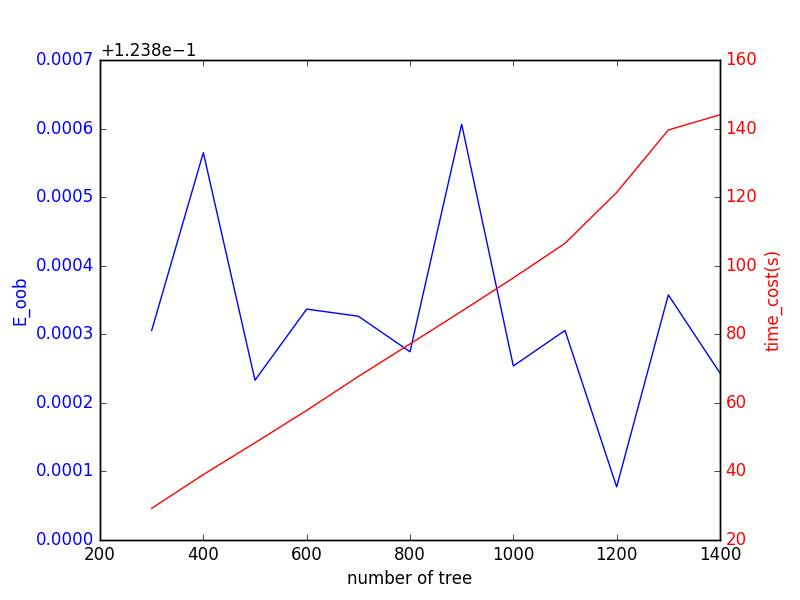
\includegraphics[width=1.0\linewidth]{RF-1.jpg}
		\caption{number of trees}
		\label{rf-1}
	\end{subfigure}
	\begin{subfigure}{.4\textwidth}
		\centering
		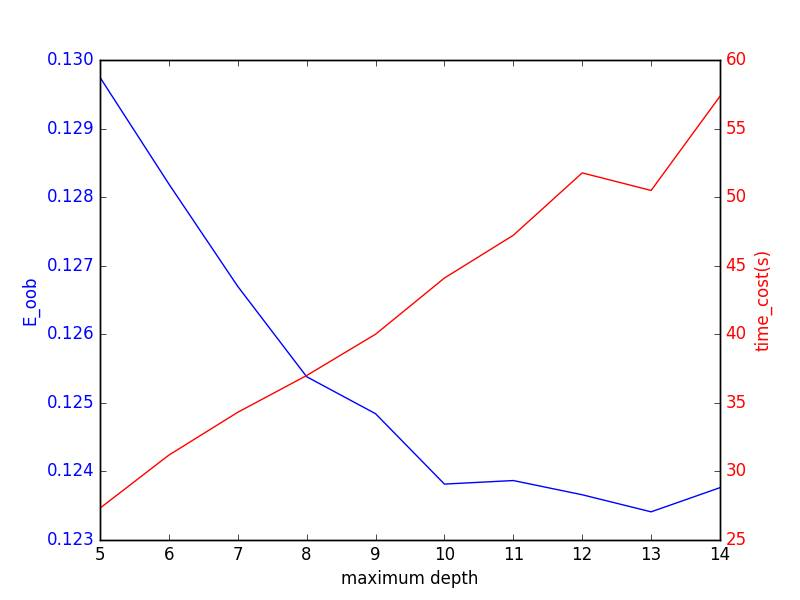
\includegraphics[width=1.0\linewidth]{RF-2.jpg}
		\caption{maximum depth}
		\label{rf-2}
	\end{subfigure}
	\caption{out-of-bag error versus time spent}
\end{figure}
\begin{enumerate}
	\item number of trees
	
	From figure (\ref{rf-1}) we can find that as the number of trees increases, the time spent during the training increases steadily but the out-of-bag error goes up and down. Consequently, there is no need to use too many trees, and we choose to use 1000 as the number of trees.
	\item regularization of trees
	
	From figure (\ref{rf-2}) we can find that as the maximum depth increases, out-of-bag error decreases and time spent during the training increases. However, because the growing rate of time is higher than the decreasing rate of out-of-bag error,we choose to use 10 as the maximum depth of each tree.
\end{enumerate}

\subsubsection{About the Use of Training Data}

Because we have lots of features in our training and testing data(55 in total),we decide to remove those unimportant features during training. First,we use the \url{feature_importances_} function in RandomForestClassifier of SKLearn to get the relative importance of each feature; then we check the performance of Random Forest after removing some unimportant features and decide the optimal number of removals, according to the attribute \url{oob_score} in Random-ForestClassifier.We discover that removing the two least important features will increase the performance of the classifier.

\subsection{Uniform aggregation of Gaussian Kernel Logistic Regression}

In this final project, we also try kernel logistic regression as the model as consideration. Since we aim to find an method that can predict the probability as target for effetely and large model complexity, we choose logistic regression with gaussian kernel as our model. 

However, in order to reduce memory usage and computation time, we divided the training data into 6 part, and trained 6 GKLR (Gaussian Kernel logistic regression separately), then use the uniform aggregation to blend them all. 

The model are shown in following diagram. First one is the training phase and the second one is the prediction phase. We use 90000 data as training data and 6434 data as validation data, and each KLR are training with 15000 data separately.
\begin{figure}[H]
	\centering
	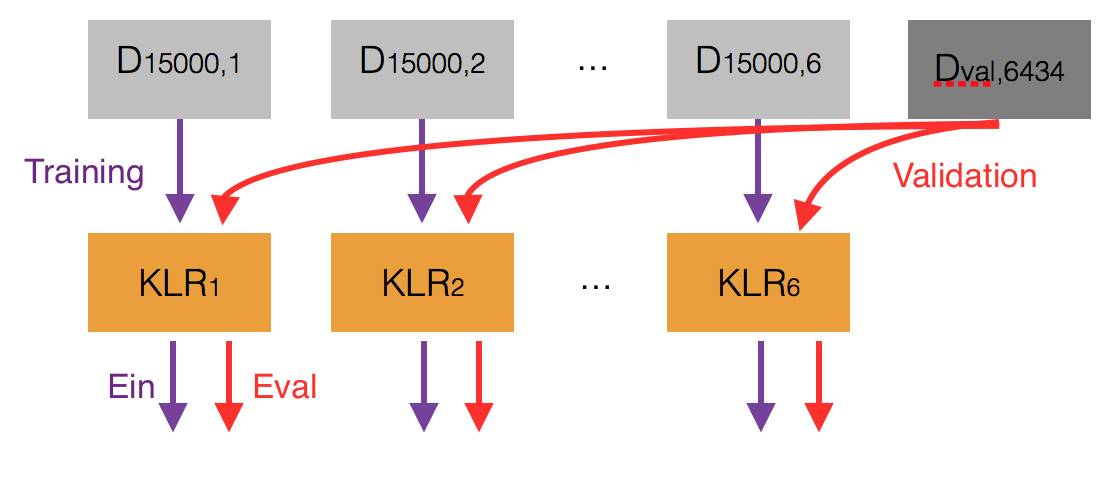
\includegraphics[scale=0.3]{KLR-1.png}
	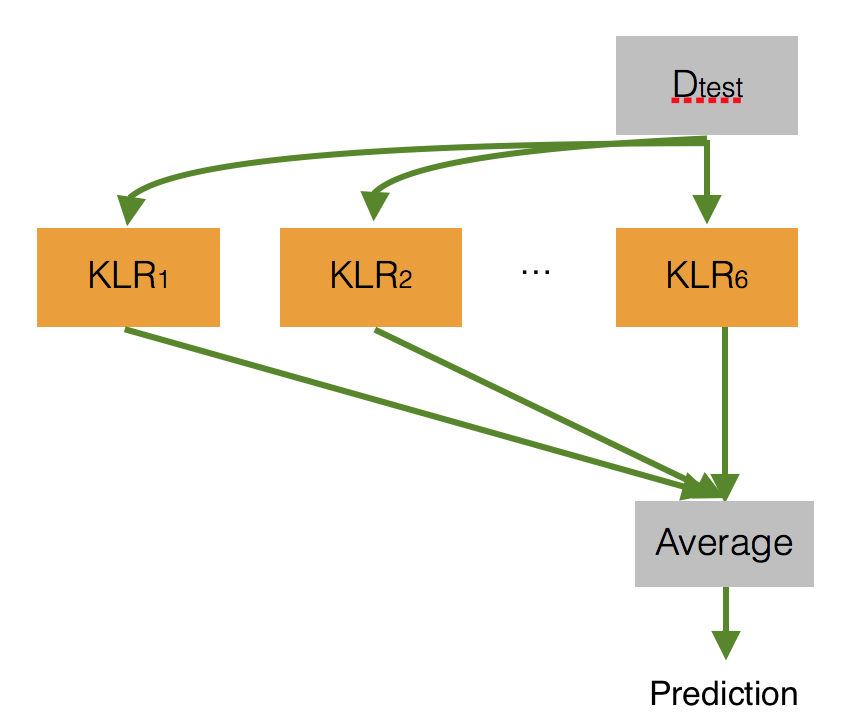
\includegraphics[scale=0.3]{KLR-2.png}
\end{figure}
In the prediction phase, the 6 KLR models are aggregate uniformly to prediction an probability.
Note that, we have to decide two parameter is this model. First is the “lambda” constant for the L2-regularizer penalty, Second is the “gamma” constant of the gaussian kernel. We try different parameter and select the best one of good validation error. 

\subsubsection{Equation}

\begin{align}
\min_{\beta}\SBrackets{\lambda\bm{\beta}^T\BF{K}\bm{\beta}+\sum_{n=1}^{N}\log\ParTh{1+\exp\ParTh{-y\otimes\BF{K}\bm{\beta}}}},~\BF{K}_{m,n}=\exp\ParTh{-\gamma\VecAbsVal{\BF{x}_m-\BF{x}_n}^2}
\end{align}

\subsubsection{Validation Result : (with 55 features)}

\begin{figure}[H]
	\centering
	\begin{subfigure}{.4\textwidth}
		\centering
		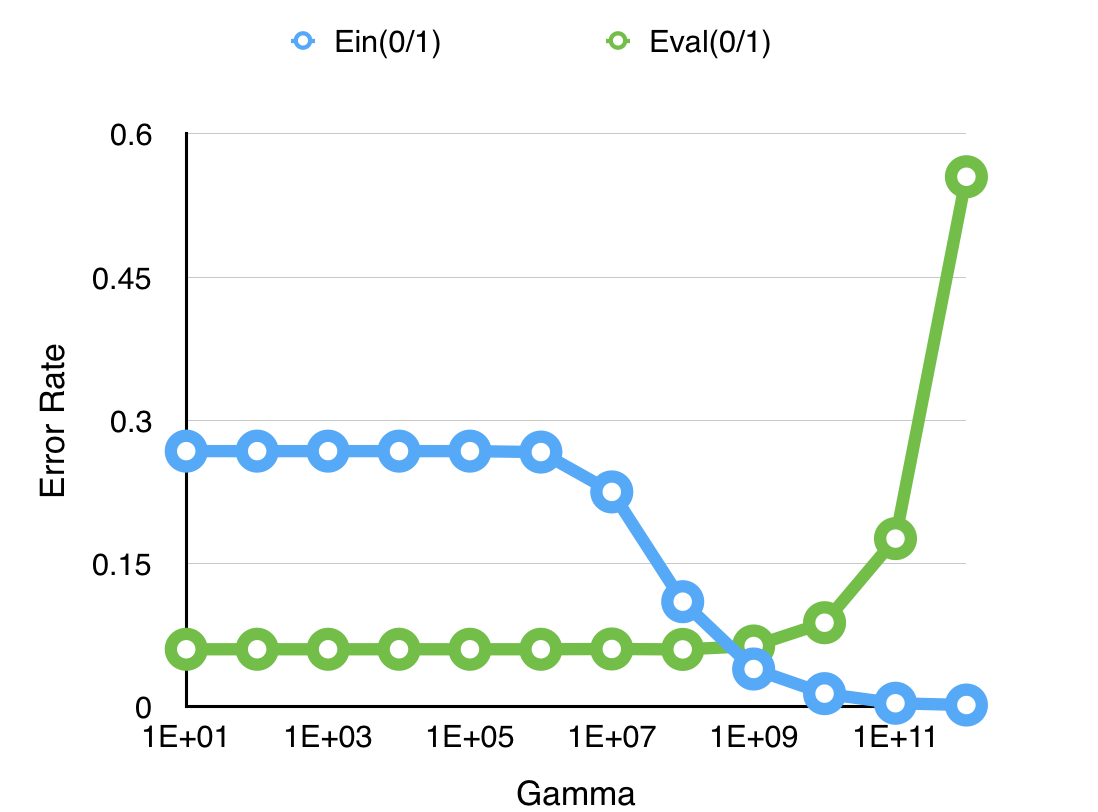
\includegraphics[width=1.0\linewidth]{KLR-3.png}
		\caption{Changing $\gamma$}
	\end{subfigure}
	\begin{subfigure}{.4\textwidth}
		\centering
		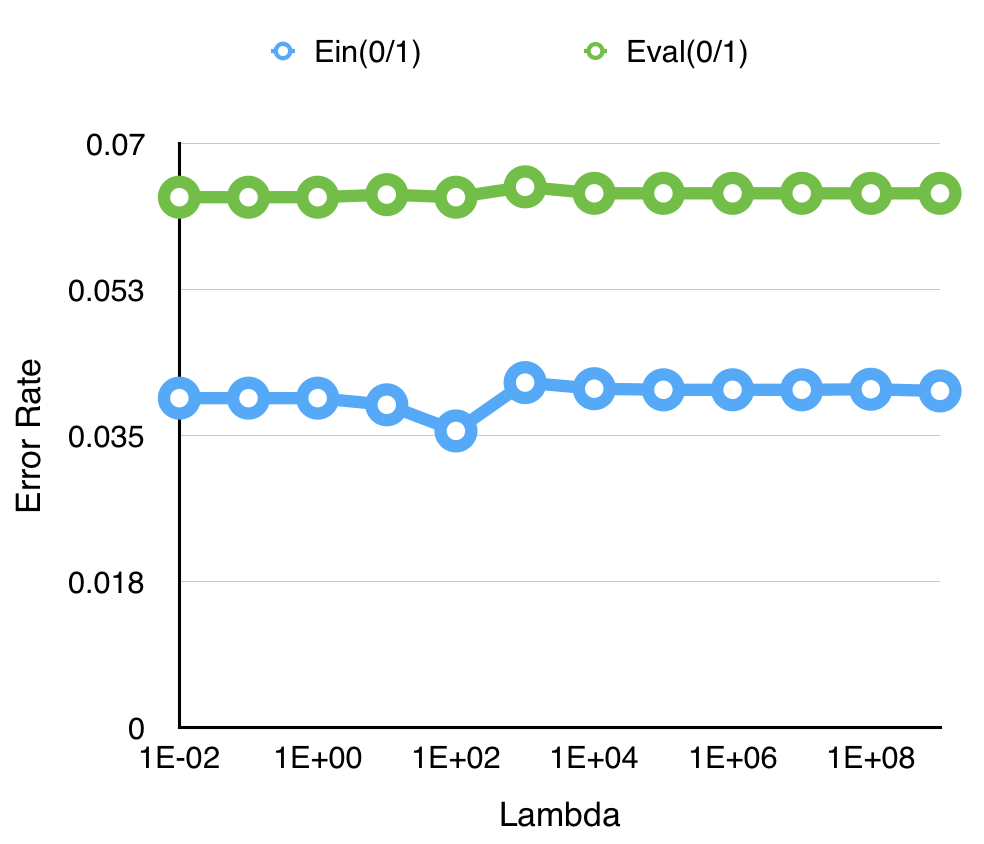
\includegraphics[width=1.0\linewidth]{KLR-4.png}
		\caption{Changing $\lambda$}
	\end{subfigure}
\end{figure}

\subsubsection{Discussion}

From figure above, we can see that with gamma equal ${10}^9$, the model have less validation error. Also, with Lambda equal ${10}^2$, the model have less in-sample error. As a result, we choose gamma to be ${10}^9$ and Lambda to be ${10}^2$.

\subsection{Gradient Tree Boosting}

Here I used the \url{sklearn.ensemble.GradientBoostingClassifier}.

\subsubsection{Pros of Gradient Tree Boosting}

\begin{enumerate}
	\item Efficiency
	\item Predictive power
	\item Robustness to outliers in output space
\end{enumerate}

\subsubsection{How to Choose Parameters}

\begin{figure}[H]
	\centering
	\begin{subfigure}{.4\textwidth}
		\centering
		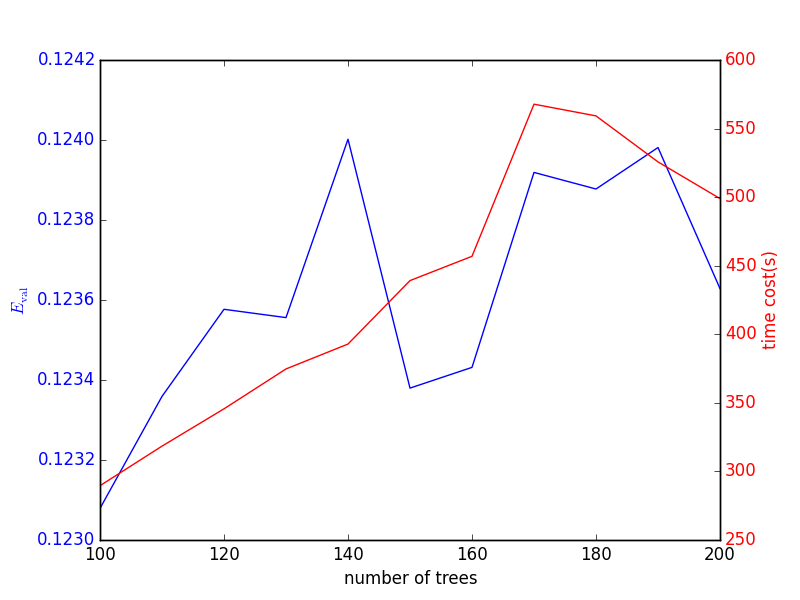
\includegraphics[width=1.0\linewidth]{GB-1.png}
		\caption{number of trees}
		\label{gb-1}
	\end{subfigure}
	\begin{subfigure}{.4\textwidth}
		\centering
		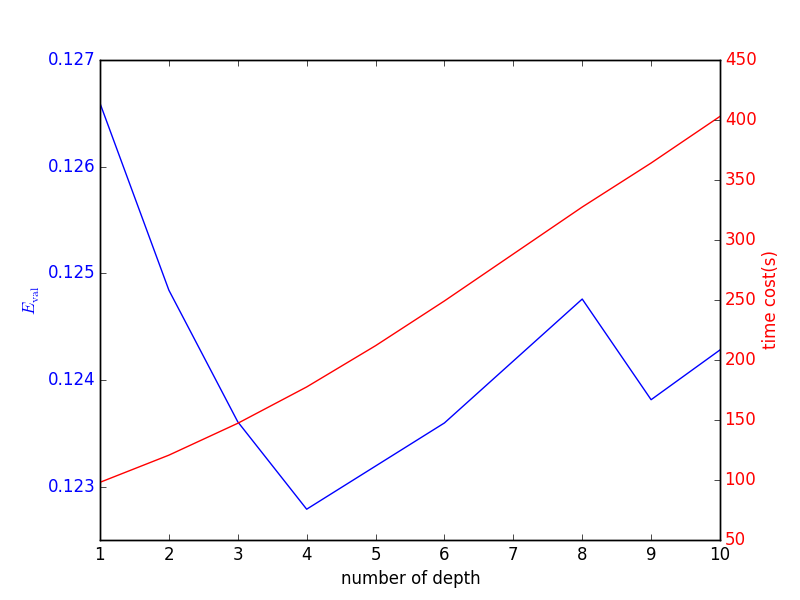
\includegraphics[width=1.0\linewidth]{GB-2.png}
		\caption{number of depth}
		\label{gb-2}
	\end{subfigure}
	\caption{$E_{\text{val}}$ v.s. time costs}
\end{figure}
From figure (\ref{gb-1}) we see that $E_{\text{val}}$ number of trees grows as number of trees increases. So we choose 100 to be the number of trees.

From figure (\ref{gb-2}) we can see that the best $E_{\text{val}}$ is around 4 depth, we choose depth to be 6 finally.

\subsubsection{Some Other Pre-processing Before Training}

By using the attributes \url{feature_importances_} of this model, we removed first two not important features to enhance our performance. This attribute will show the score of each feature. After removing the features, we start to train the model.

\section*{Reference}

\begin{enumerate}

\item[{[1]}] Lecture Notes by Hsuan-Tien LIN, Department of Computer Science and Information Engineering, National Taiwan University, Taipei 106, Taiwan.

\item[{[2]}] sklearn: \url{http://scikit-learn.org/}

\item[{[3]}] TensorFlow: \url{https://www.tensorflow.org/}

\end{enumerate}

\end{document}